\documentclass[11pt]{article}


\usepackage{mathptmx}
\usepackage[T1]{fontenc} 

\usepackage{lipsum}
\usepackage[margin=1in,left=1.5in,includefoot]{geometry}   

\usepackage[hidelinks]{hyperref} % Allows for clickable references // hidelinks --> stops links from being formatted differently

\usepackage{color} 
\usepackage{xcolor}

% Graphics preamble 
\usepackage{graphicx} %Allows to import images 
\usepackage{float} %Allows for control of float positions 
\graphicspath {{figures/}}  
\usepackage{wrapfig}
\usepackage{subcaption}


% Text preamble
\usepackage[normalem]{ulem} %underlining 
\newcommand{\myparagraph}[1]{\paragraph{#1}\mbox{}\\} 

%Table Preamble
\usepackage{pbox}


% Source Code preamble
\usepackage{listings} %code highlighter
\usepackage{color} %use color
\definecolor{mygreen}{rgb}{0,0.6,0}
\definecolor{mygray}{rgb}{0.5,0.5,0.5}
\definecolor{mymauve}{rgb}{0.58,0,0.82}
 
%Customize a bit the look
\lstset{ %
backgroundcolor=\color{white}, % choose the background color; you must add \usepackage{color} or \usepackage{xcolor}
basicstyle=\tiny, % the size of the fonts that are used for the code  
breakatwhitespace=false, % sets if automatic breaks should only happen at whitespace
breaklines=true, % sets automatic line breaking 
captionpos=b, % sets the caption-position to bottom
commentstyle=\color{mygreen}, % comment style
deletekeywords={...}, % if you want to delete keywords from the given language
escapeinside={\%*}{*)}, % if you want to add LaTeX within your code
extendedchars=true, % lets you use non-ASCII characters; for 8-bits encodings only, does not work with UTF-8
frame=single, % adds a frame around the code
keepspaces=true, % keeps spaces in text, useful for keeping indentation of code (possibly needs columns=flexible)
keywordstyle=\color{blue}, % keyword style
% language=Octave, % the language of the code
morekeywords={*,...}, % if you want to add more keywords to the set
numbers=left, % where to put the line-numbers; possible values are (none, left, right)
numbersep=5pt, % how far the line-numbers are from the code
numberstyle=\tiny\color{mygray}, % the style that is used for the line-numbers
rulecolor=\color{black}, % if not set, the frame-color may be changed on line-breaks within not-black text (e.g. comments (green here))
showspaces=false, % show spaces everywhere adding particular underscores; it overrides 'showstringspaces'
showstringspaces=false, % underline spaces within strings only
showtabs=false, % show tabs within strings adding particular underscores
stepnumber=1, % the step between two line-numbers. If it's 1, each line will be numbered
stringstyle=\color{mymauve}, % string literal style
tabsize=2, % sets default tabsize to 2 spaces
title=\lstname % show the filename of files included with \lstinputlisting; also try caption instead of title
}
%END of listing package%
 
\definecolor{darkgray}{rgb}{.4,.4,.4}
\definecolor{purple}{rgb}{0.65, 0.12, 0.82}
 
%define Javascript language
\lstdefinelanguage{JavaScript}{
keywords={typeof, new, true, false, catch, function, return, null, catch, switch, var, if, in, while, do, else, case, break},
keywordstyle=\color{blue}\bfseries,
ndkeywords={class, export, boolean, throw, implements, import, this},
ndkeywordstyle=\color{darkgray}\bfseries,
identifierstyle=\color{black},
sensitive=false,
comment=[l]{//},
morecomment=[s]{/*}{*/},
commentstyle=\color{purple}\ttfamily,
stringstyle=\color{red}\ttfamily,
morestring=[b]',
morestring=[b]"
}
 
\lstset{
language=JavaScript,
extendedchars=true,
basicstyle=\footnotesize\ttfamily, 
showstringspaces=false,
showspaces=false,
numbers=left,
numberstyle=\footnotesize,
numbersep=9pt,
tabsize=2,
breaklines=true,
showtabs=false,
captionpos=b
}



% Table preamble
\usepackage{array}


%Math preamble
\usepackage{mhchem} %Allows us to write chemistry equations! 
\usepackage{xfrac} % Allows for slanted fractions 


% Bibliography preamble
\usepackage[numbers,sort&compress]{natbib} %Sorts references by numner, if 1,2,3 --> 1-3 is shown

% Bullet preamble 
\renewcommand{\labelitemi}{$\bullet$}  
\renewcommand{\labelitemii}{$\diamond$}  
\renewcommand{\labelitemiii}{$\circ$}      

% Header and Footer Stuff
\usepackage{fancyhdr}
\pagestyle{fancy}
\fancyhead{}
\fancyfoot{}
\fancyfoot[R]{\thepage}     
\renewcommand{\headrulewidth}{1pt}  
\renewcommand{\footrulewidth}{1pt}     
  
 

\setcounter{section}{0}  
\setcounter{tocdepth}{2}
\setcounter{secnumdepth}{4} 
 
\begin{document}

\begin{titlepage} 
	\begin{center}
	\line(1,0){300} \\
	[4mm]
	\huge{\bfseries WT1 Webapplications \\ NoSQL Databases} \\
	[2mm]
	\line(1,0){200}\\	
	[1.5cm]
	\textsc{\LARGE HTW BERLIN}\\
	[0.75cm]
	\textsc{\LARGE Internationale Medieninformatik} \\  
	[9cm]
	\end{center}	 
	\begin{flushright}
		\textsc{\large Jakub Mueller / David Schmoecker / Jonas Heinig \\
		544832 / 544655 / 550169 \\
		WS18/19\\}
	\end{flushright} 
	 
	
	
\end{titlepage}  
 
% Front matter stuff
\pagenumbering{roman} 

% Table of Contents Stuff
\tableofcontents
  
\cleardoublepage %Make section start on next page 




% Main Body Stuff 
\pagenumbering{arabic} 
\setcounter{page}{1} %Reset page counter to 1 (to make page with first section start on page 1 instead of ...) 



\section{Brief look into History} 
In 1998 the term NoSQL was first used by Carlo Strozzi while naming his open-source "relational" database that did not use SQL. In this context the meaning of the acronym NoSQL was "no SQL".
In early 2009 Johan Oskarsson reintroduced the term NoSQL when he organized an event to discuss "open source distributed, non relational databases". The acronym NoSQL becomes a term to classify the movement of non-relational, distributed data stores. So the meaning changed from "no SQL" to "not only SQL".
These non-relational systems were called "Document-oriented databases" before. Most of the early NoSQL systems did not attempt to provide atomicity, consistency, isolation and durability guarantees,  contrary to the prevailing practice among relational database systems (ACID).
NoSQL systems are more popular than ever before but relational databases are still dominating the market.  


\section{Terminology}
The terminology in NoSQL databases are slightly different compared to relational models. Below are some changed terms with a short description: 

	\begin{figure}[H]
		\centering 
		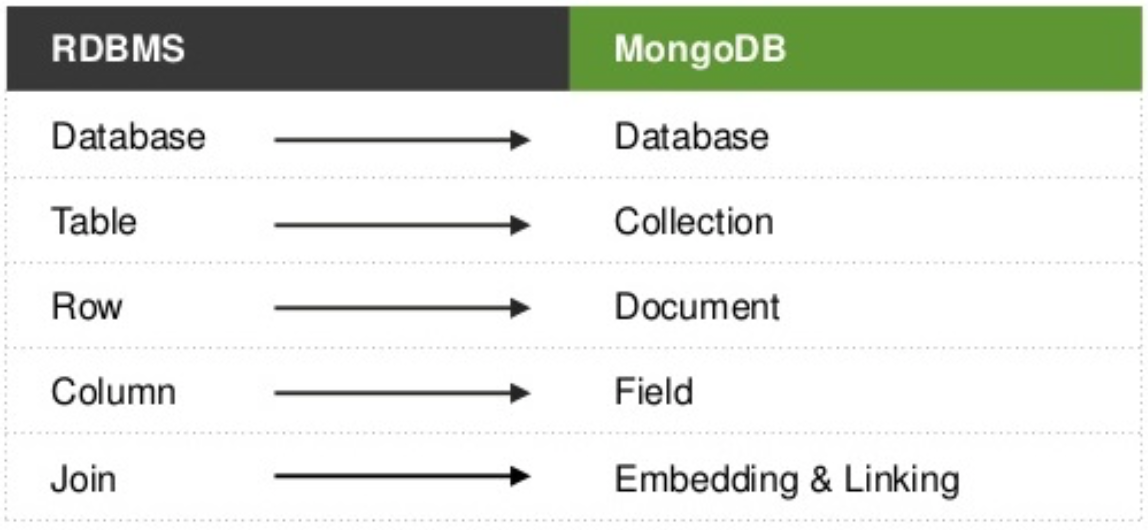
\includegraphics[height=4cm]{figures/terminology}     
		\caption{Terminology}          
	\end{figure}   


A table or relation is defined as a set of tuples (rows) that have the same attributes (columns). A tuple usually represents an object and information about that object. Objects are typically physical objects or concepts. A relation is usually described as a table, which is organized into rows and columns. All the data referenced by an attribute are in the same domain and conform to the same constraints. 


	\begin{figure}[H]
		\centering 
		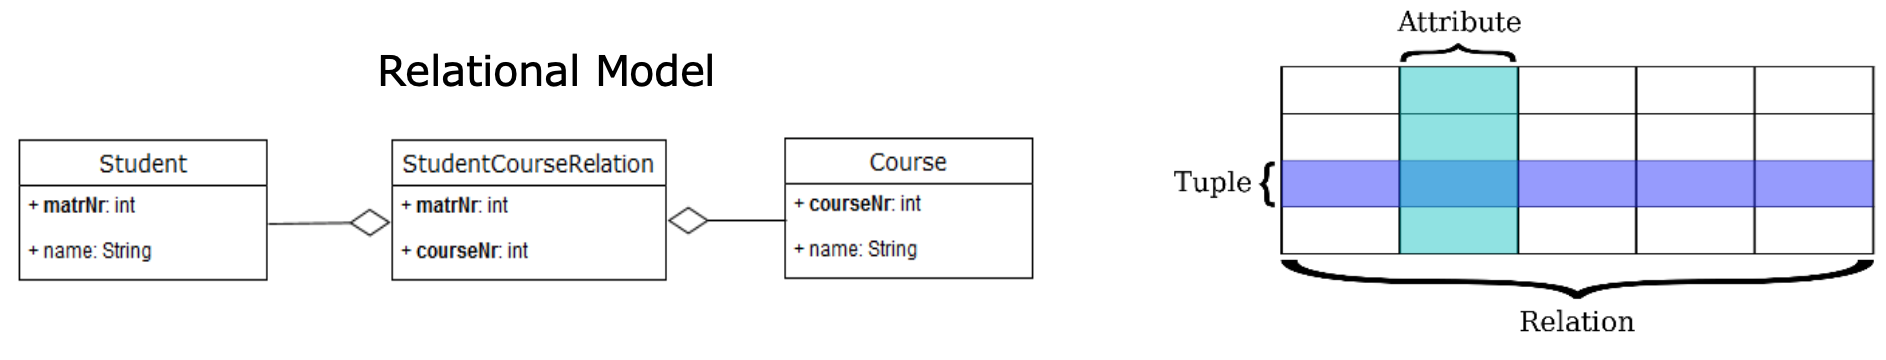
\includegraphics[height=3cm]{figures/relational-model}     
		\caption{Relational Model}          
	\end{figure}   


\cleardoublepage

NoSQL databases like MongoDB using collections instead of tables. A collection stores different objects with the same attributes. A collection is a set of documents, so these objects are represented as a single document in the collection.

	\begin{figure}[H]
		\centering 
		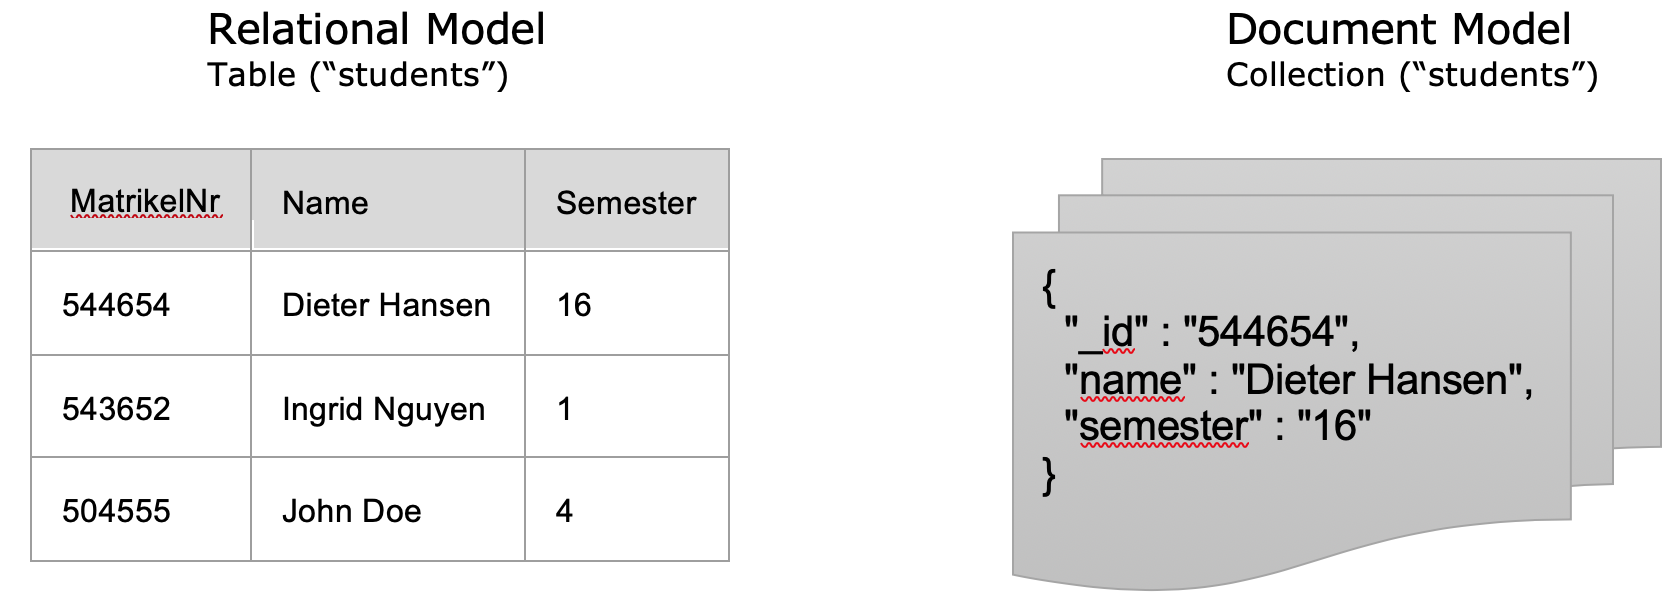
\includegraphics[height=3cm]{figures/relational-document}     
		\caption{Table vs. Collection}           
	\end{figure}   


These documents represent one row in the table. So one document is one object containing the information, split in columns which are the attributes. In relational models it is common to combine different tables with a "join", to get the needed information.
Instead of joining different tables, MongoDB provides the possibility to embed or link documents to create a relation between documents in different collections.    

	\begin{figure}[H]
		\centering 
		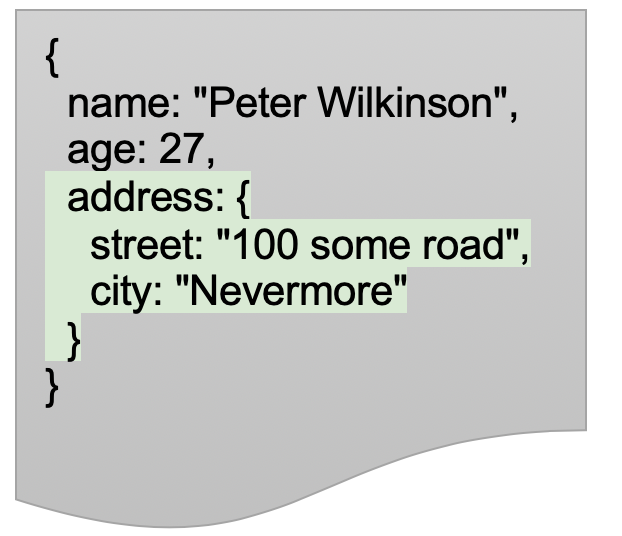
\includegraphics[height=3cm]{figures/embedded-address}     
		\caption{Embedding}           
	\end{figure}    

You can embed an object into another object,
If you add a field to your object, 
which contains another object.
Here you can see a document of "user",
where another object was added
to store and access the address of the user. 

Another way to store and access the address of a specific user, is to link both documents with a foreign key. You just have to write the key of the user as foreign key into the document of the address.


	\begin{figure}[H]
		\centering  
		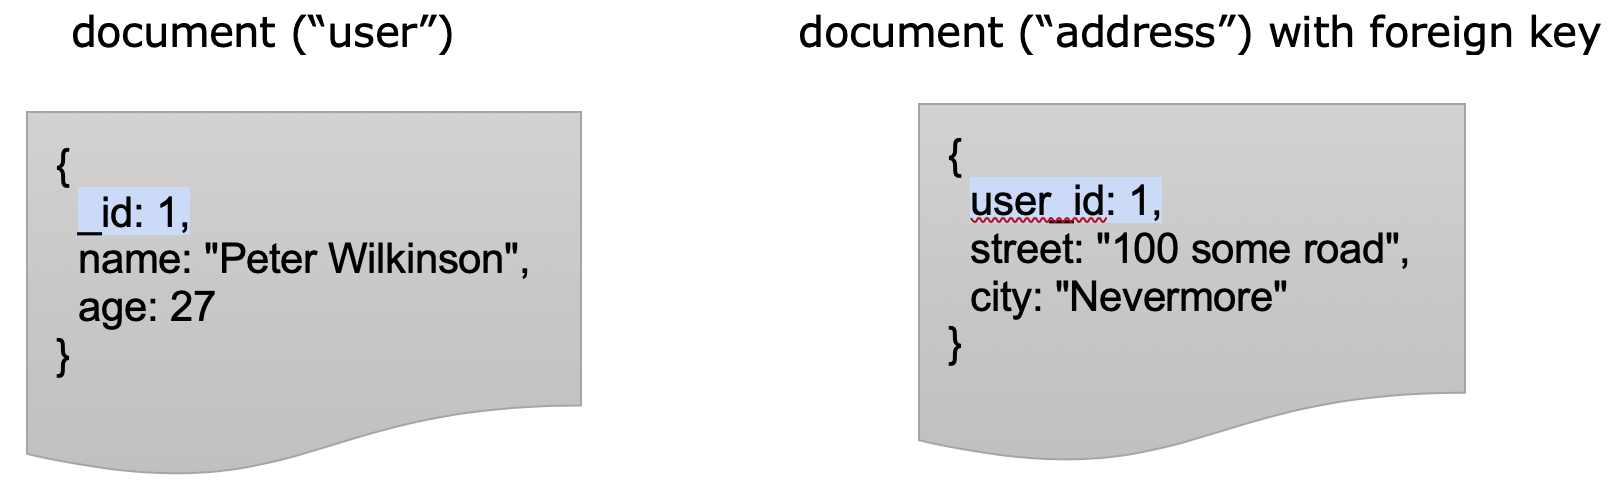
\includegraphics[height=3cm]{figures/linking}     
		\caption{Linking}           
	\end{figure}     

 
\section{Types of NoSQL databases} 
Just as the term "Not only SQL" is pretty broad, there are a broad variety of different database-systems to which it applies.
Many of these different systems can be categorised in one of the following four general types. \cite{nosqllist}

\subsection{Key-Value pair based databases}
Key-Value pair based databases are the simplest type of NoSQL databases. 
As the name suggests they store key-value pairs. 
The key is a unique string which is also the only way to query the database.\cite{kvquery} 
The value on the other hand can be anything: a string, a number, a JSON document or even an entire new set of key-value pairs encapsulated in an object. 
Known key-value pair based databases are Amazon's DynamoDB and the open source database Riak. 
\subsection{Document databases}
Document databases also called document store collections of documents that include the data to be saved. 
Depending on the specific database these documents have different encodings like for example XML, YAML or JSON. 
They are similar to Key-Value pair based databases. 
One key difference is that the content of the documents are used for queries. 
Next to MongoDB another well known document database is Apache CouchDB.

\subsection{Graph databases}
Graph databases are based on Graphs which consist of Nodes and Edges. A node represents and entity and edges represent relationships between those entities. This makes them suitable to model highly interconnected data, which other No-SQL databases struggle with. \\
Some graph databases use native graph storage that is optimised and designed for storing and managing graphs, others serialize the graph data into a relational, object-oriented database, or some other general-purpose data store. \cite{graph_storage}

\subsection{Column based databases}
Column databases are based on tables just as relational databases. They use a different approach that is column oriented.
They store each column separately to allow for quicker scans when only a small number of columns are involved. 
\cite{columnbased} 
\begin{figure}[H]
	\centering 
	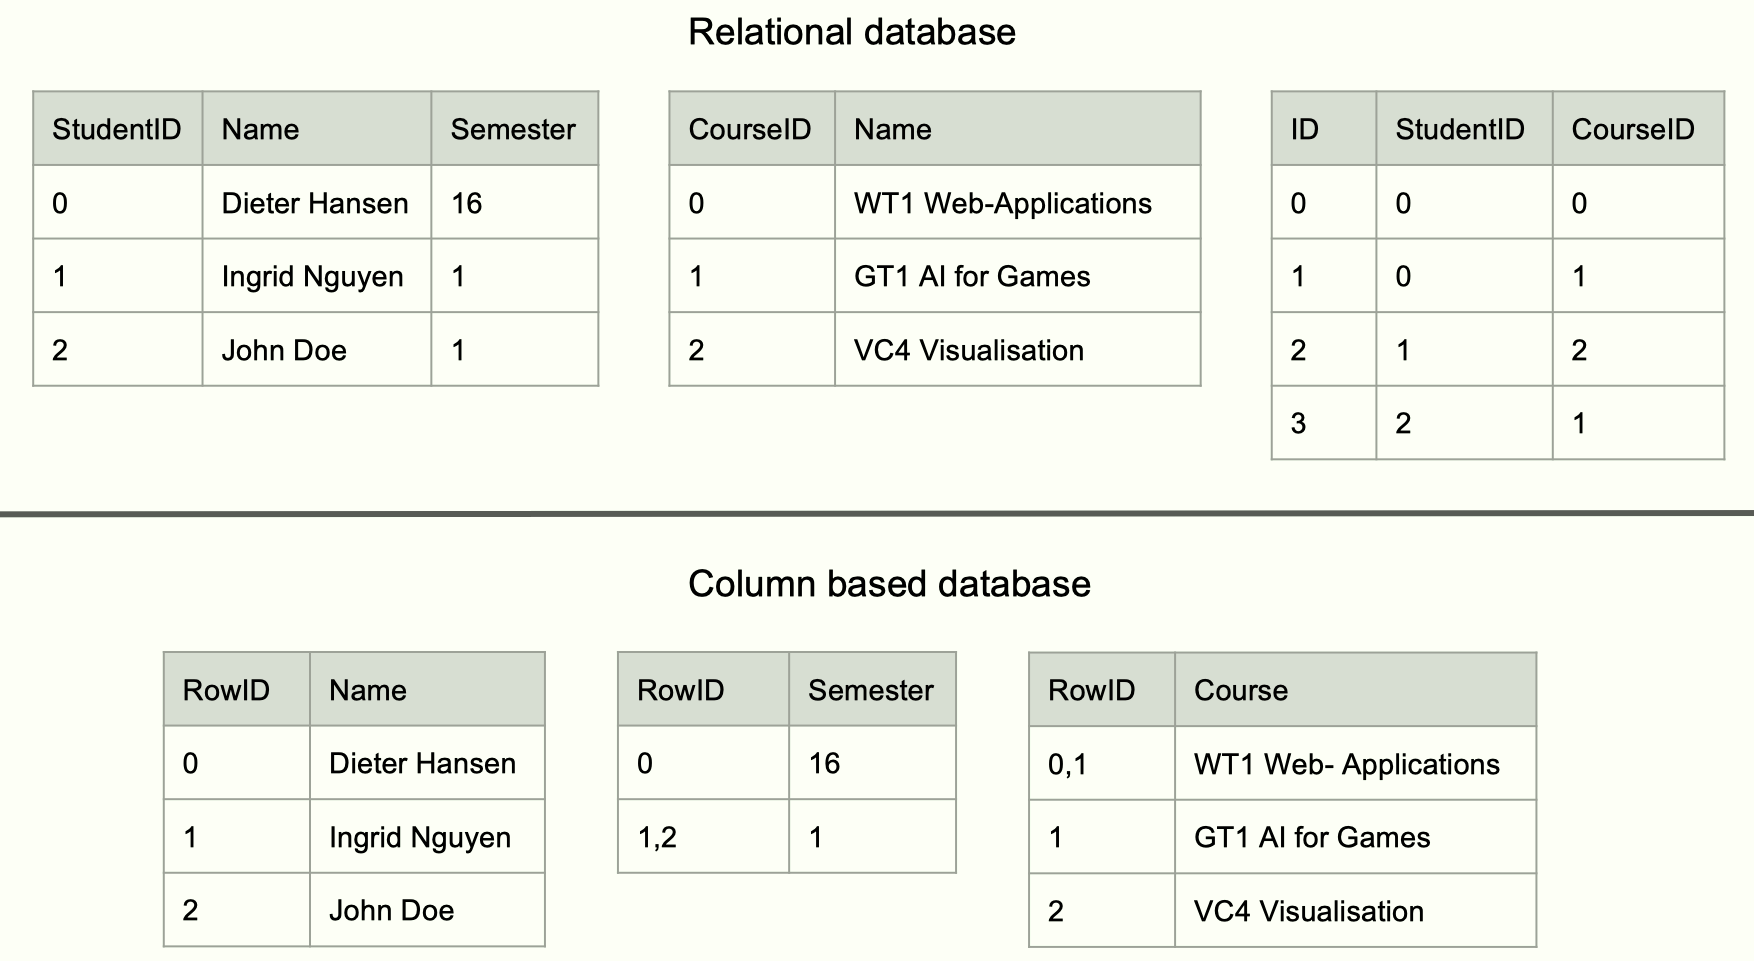
\includegraphics[height=8cm]{figures/column_based}     
	\caption{Standard relational and column based layout of tables that hold the same data}          
\end{figure}   
Examples for this type of databases are Apache Cassandra (which was developed by Facebook) and Google's Big Tables.
\section{MongoDB} 
MongoDB is a very poplar and well supported open source No-SQL database. The main difference between traditional relational databases is that No-SQL databases do not store their data in tables, but rather in collections that are stored in JSON. Since JSON is the default object notation for JavaScript it works great with that language and makes development fast, efficient and easy. In general No-SQL databases claim to be highly scalable, efficient on storage, easily manageable and easy in their initial setup. On the contrary they often offer less functionality, are not so well-supported and there are not as many developers out there who can call themselves experts on the topic. 
	In general it can be said that No-SQL databases are a good choice when dealing with modern Web 2.0 applications, while they might not be the way to go when developing on different ground. \cite{nosqladvantages} The following chart gives a basic overview about some differences and similarities between SQL and No-SQL databases. 
	

\begin{table}[H]
\begin{tabular}{|c|c|c|}
\hline
                      & SQL                                                                                                      & No-SQL                                                                                             \\ \hline
Both have a           & Database                                                                                                 & Database                                                                                           \\ \hline
Structure of Database & Table                                                                                                    & Collection                                                                                         \\ \hline
Entity               & 1 Row inside the table                                                                                   & \begin{tabular}[c]{@{}c@{}}1 Document inside \\ the collection\end{tabular}                        \\ \hline
Entity Structure      & \begin{tabular}[c]{@{}c@{}}Table contains the same \\ properties (columns) for all entities\end{tabular} & \begin{tabular}[c]{@{}c@{}}Properties may vary between \\ documents in the collection\end{tabular} \\ \hline
\end{tabular}
	\caption{SQL and No-SQL Databases} 
	\label{tab:SQL and No-SQL Databases} 
\end{table}




\subsection{MongoDB \_id}
The \_id property is part of every document that is stored inside MongoDB. It serves as a primary key used to identify the document. In many SQL databases an auto-incrementing integer value is used as a primary key, MongoDB on the other hand uses a generated 12 byte value such as 507f1f77bcf86cd799439011. The \_id is generated in the following way:

\begin{itemize}
	\item First 4 bytes: Timestamp referring to moment in time the document was created
	\item Next 3 bytes: Machine-Identifiers. These make sure that 2 machines can insert at the exact same time without conflicts
	\item Next 2 bytes: Process-ID serves as another way to create unique identifiers
	\item Last 3 bytes: Counter, similar to what MYSQL would do
\end{itemize} 

Even though it is not necessary nor recommended in most cases, we may change the \_id property of any document to whatever we like without breaking anything. 






\subsection{Working with MongoDB}

\noindent
\textbf{Adding a  Document to the Database} \\  
Adding a document to a MongoDB database is as easy as calling a method on the database instance. If the instance we are referencing has not been created at this point, MongoDB will automatically create it for us.  

\begin{lstlisting}
db.collection("Tasks").insert({content: "Eat Lunch", done: false}).then((result) => {
  console.log(result);
})
\end{lstlisting}

\noindent
\textbf{Getting a  Document from the Database} \\  
In order to query data from a MongoDB collection we can use the built in find method. When we call the find method without providing any arguments all documents in the collection will be returned in an unstructured way. 
 
\begin{lstlisting}
db.collection("Tasks").find().then((result) => {
  console.log(result); //Will print all documents
})
\end{lstlisting}

When we would only like to receive a single item we simply have to pass in some criteria to the find method. In the example below we would like to receive a document from the collection that has a content property with a value of "Eat Lunch". 

\begin{lstlisting}
db.collection("Tasks").find({content: "Eat Lunch"}).then((result) => {
  console.log(result);
})
\end{lstlisting}

\noindent
\textbf{Deleting Documents from Database} \\  
The deleteMany method can be used to delete all documents that fit the criteria we pass in. In this example we are deleting all documents that have a content property with the value "Eat Lunch". 

\begin{lstlisting}
db.collection("Tasks").deleteMany({content: "Eat Lunch"}).then((result) => {
  console.log(result);
})
\end{lstlisting}

On the contrary we have the deleteOne method if we would only like to remove the first item from the database that matches our criteria. When an item has been found the method immediately stops. 
\begin{lstlisting}
db.collection("Tasks").deleteOne({content: "Eat Lunch"}).then((result) => {
  console.log(result);
})
\end{lstlisting}


The findOneAndDelete method works very similar to the previous one. Though the difference is that it does not only delete the first item that matches but also returns it. In this case we are deleting the first document that has a property done with the value false. 

\begin{lstlisting}
db.collection("Tasks").findOneAndDelete({done: false}).then((result) => {
  console.log(result);
})
\end{lstlisting}

When we would like to delete a document by its unique identifier we have to create a new ObjectID by providing the id string value of the document to the ObjectID constructor and pass it into our findOneAndDelete method. This can be done in the following way. 

\begin{lstlisting}
...
var ObjectID = mongoose.Schema.Types.ObjectId;
...
db.collection("Users").findOneAndDelete({_id: new ObjectID("5af6e4721342c78d496ddce6")}).then((result) => {
  console.log(result);
})
\end{lstlisting}  

\noindent
\textbf{Updating Documents in the Database} \\  

When updating documents inside MongoDB we can use MongoDB's built in update operators to simplify the process. A complete list of all update operators can be found at \url{https://docs.mongodb.com/manual/reference/operator/update/}. The example below demonstrates a basic update tasks. We call the findOneAndUpdate method to update a value in a document using the built in update operator \$set. In this case we want to set the done property of the matching element to true. 

\begin{lstlisting}
db.collection("Tasks").findOneAndUpdate({
    _id: new ObjectID("5afb4d7d924f0d0154a3c27e")
  }, {
      $set: {
        done: true
      }
    }, {
      returnOriginal: false //prevents returning the original document and returns the updated one instead
  }).then((result) => {
    console.log(result);
 });
\end{lstlisting}
 

\subsection{Sharding and Replication}
Sharding and replication are database-concepts that will provide higher write performance and increase fault tolerance respectively. Furthermore, by using either of the two, higher read speeds can be achieved. 
They are not exclusive to No-SQL databases but are usually more complex to use with RDMBS and commonly require extra software. 
MongoDB has the functionality built-in. Both concepts make use of multiple instances or systems running MongoDB. 
Replication uses multiple systems that have the same data, while sharding partitions the data between different machines. 
\subsubsection{Replication}

In MongoDB there are two types of replication: \textit{master-slave replication} and \textit{replica sets}. Both are based on the operations log (\textbf{oplog}).
The operations log is a special collection that records all operations that add, delete or modify data in the database. 
It's a capped collection, which means that when it grows over a specified size it will start deleting older entries. 
When applying all steps in a complete operations log, on an empty database, it will afterwards be in the same state. 
That's the base concept for both types of replication. 
In master-slave replication systems there is one master that will run all operations that modify the data. The slaves will repeat all steps from the oplog of the master.
Slaves will thus be in the same state as the master and can be queried, thus increasing the read speed. There cannot be made any changes to the data using the slave systems.
In case that the master node goes offline, the data is not lost and the system reads can still be executed.
Replica-sets are similar to the master-slave system, but have automatic-failover. There is a primary node that acts similar to the master and secondary nodes that are similar to the slaves. 
The difference is that in case the primary node goes offline, the system will make a secondary node the new primary node. It will still be able to run all queries. 

%TODO add sample code for master-slave

\subsubsection{Sharding}
Through Sharding MongoDB supports \textit{horizontal scaling}, meaning that instead of increasing the capacity of one computer, like using a better CPU or adding more RAM (\textit{vertical scaling}), more machines are added and the data is split between them. MongoDB is designed to be able to scale out easier than RDBMS but still it is a difficult and complex way to configure sharding on MongoDB and should be well thought through.
\cite{designed_to_scale}
So sharding should only be used if required and can be activated on systems that run initially without it. 
How to distribute the data to different machines is a core question when considering sharding.
\paragraph{Manual vs automatic sharding} \mbox{}\\
Sharding is possible by simply defining a rule that states what data gets do be stored on what system.
Finding such a rule depends on the data and the application. 
For this simple example imagine a company that saves some data about its users including their names. The company acquired so many users that they don't fit on one system anymore, so they decide to split the data to three servers. 
A possible rule would be to save the data of the users depending on the first letter of their last name. A-I on the first, J-R on the second S-Z on the third system. 
The application that uses a system like this would need to know where to look for or add a user. This is not very flexible and adds complexity to some tasks. 
To get the total number of users, three different queries would now be necessary. Also there is no guarantee that the data will be spread evenly on the systems. 
This is an example for manual sharding and can be done with any database.
Automatic sharding as it is implemented in MongoDB allows your application to ignore the fact that it isn't talking to only one MongoDB server, to some extent. 
It also automates balancing the data across the different systems. 
\cite{automatic_sharding}

\paragraph{Shard keys} \mbox{}\\
Sharding in MongoDB can be controlled on the collection level, meaning that one collection might be split up onto different systems and others might reside on a single one.
A collection will be split into chunks, which will be saved on the different shards.
The decision on what chunks go onto what shard, is made using the shard key of the collection. 
This key consists of an immutable field or fields that exist in every document in the collection and cannot be changed later. 
Chunks have a range of the data they contain based on the shard key.
\cite{shard_keys}

\paragraph{Router} \mbox{}\\
The interface that applications talk to when using sharding is an instance of \textbf{mongos} instead of talking directly to the shards. 
The router in MongoDB routes queries and write operation to shards. 
\cite{router}
It's also used for configuration tasks like adding or enabling shards.

\paragraph{Necessary setup steps}\mbox{}\\
To set up sharding for a collection the following steps are necessary:

\begin{enumerate}
	\item Starting the shards as standard mongod-processes 
    \item Defining the shard key for the collection to be sharded \\
    This can be done using \textit{sh.shardCollection()}
    \item Starting a router and adding shards \\
    Shards can be added using \textit{sh.addShard()}
	\item Enabling sharding on the router \\
	This can be done using \textit{sh.enableSharding()}
\end{enumerate}
   


\section{Mongoose}
"Mongoose provides a straight-forward, schema-based solution to model your application data. It includes built-in type casting, validation, query building, business logic hooks and more, out of the box." \cite{mongooseintro} It is an npm library for MongoDB that simplifies development and reduces the amount of code we need to write. We can structure our data and use custom validators to ensure a clean and consistent database. Furthermore, the built in object relation mapping system allows quick and simple data exchange between our JavaScript applications and our databases. While MongoDB reinitialises its connection to the database for every action Mongoose keeps the connection open at all times. 


\subsection{Mongoose Models and Schemas} 
A Mongoose "Model is an object that gives you easy access to a named collection, allowing you to query the collection and use the Schema to validate any documents you save to that collection. It is created by combining a Schema, a Connection, and a collection name." \cite{mongoosemodelstackoverflow}. When a model is being created (line 3 below), we pass in a model name as well as a Mongoose Schema to use for that model.  
Mongoose schemas are used to define the basic structure of the entities inside a MongoDB collection. In a way they are very similar to the table definition in relational databases. The code snippet below defines a simplified version of the Task collection that we have created for our WeekMe Application. We have a total of four properties, each with a different datatype. In line 6 we set the content property of a task document to required, meaning that it won't be possible to save a document to the collection without setting a value here. One line further below we use a constrain to ensure that the minimum length of the content property is one character. There is a variety of constrains and validators available which can be found on the official mongoose website at \url{https://mongoosejs.com/docs/validation.html}. In line 12 and line 16 we use the default keyword to define a fallback value whenever no value is passed in. The done property of the task document obviously should default to false as most Tasks won't be completed yet when a user is submitting them to our application. In line 19 we use a mongoose ObjectId as the datatype. This is usually done when we want to reference another document in a different collection using a foreign key. In this case we reference the owner of the task by providing the primary key of a document in the users collection.      

\begin{lstlisting}
var mongoose = require("mongoose");

var Task = mongoose.model("Task", {
  content: {
    type: String,
    required: true,
    minlength: 1,
    trim: true //Removes any whitespaces in before or after the string
  },
  done: {
    type: Boolean,
    default: false
  },
  doneAt: {
    type: Number,
    default: null
  },
  _user: {
    type: mongoose.Schema.Types.ObjectId,
    required: true
  }
});

module.exports = {Todo};
\end{lstlisting} 

When the built in validators are not enough or we need to do some very specific validation we can define a custom validator in our schema. Within the user schema of the WeekMe application we use a custom validator (lines 9-12) to validate that the string value that is stored inside the email property matches basic email formatting. For this purpose we are using an npm module with the name validator, a library of string validators and sanitizers (more infos at: \url{https://www.npmjs.com/package/validator}).    


\begin{lstlisting}
var UserSchema = new mongoose.Schema({
  email: {
    type: String,
    required: true,
    lowercase: true,
    minlength: 1,
    trim: true, //Removes any whitespaces in before or after the string
    unique: true, //Can only exist once in Collection
    validate: {
      validator: validator.isEmail,
      message: '{VALUE} is not a valid email'
    }
  },
  ...
\end{lstlisting}
 




\subsection{Model Methods \& Instance Methods}
Mongoose provides us with the ability to define methods for our models as well as for the documents stored inside our collections. Model methods are defined using the statics keyword. They act on the entire collection while instance methods are defined using the methods keyword and only act on an instance within a collection. Below I added one example of each type from the WeekMe application. The findByToken method is a model method that finds and returns a user from the collection based on the token we pass in. The generateAuthToken method is an instance method that generates a unique token for an instance of a user inside the user collection. 

\begin{lstlisting}
UserSchema.statics.findByToken = function (token){
  var User = this;
  var decoded; 

  try {
    decoded = jwt.verify(token, process.env.JWT_SECRET);
  } catch (e) {
    return Promise.reject(); 
  }

  return User.findOne({
    "_id": decoded._id,
    "tokens.token": token,
    "tokens.access": "auth"
  });
};

UserSchema.methods.generateAuthToken = function () { 
  var user = this; 
  var access = "auth";
  var token = jwt.sign({_id: user._id.toHexString(), access}, process.env.JWT_SECRET);
  
  user.tokens = user.tokens.concat([{access, token}]);
  return user.save().then(() => {
    return token;
  });
};
\end{lstlisting}



\subsection{Mongoose Middleware}
"Middleware (also called pre and post hooks) are functions which are passed control during execution of asynchronous functions. Middleware is specified on the schema level and is useful for writing plugins. Mongoose 4.x has 4 types of middleware: document middleware, model middleware, aggregate middleware, and query middleware. Document middleware is supported for the following document functions. In document middleware functions, this refers to the document." \cite{mongoosemiddleware} Basically Mongoose middleware lets us run certain code before or after certain events occur (e.g. before we update a model). In the WeekMe application we define a Mongoose middleware on the schema to hash a password before saving it to the collection. This is achieved by using the .pre method and passing in a string value of "save" to tell the middleware at what event it should be executed. Similar to the way Express middleware is working we need to signal that our middleware has finished executing by calling the next() method in line 11 so that the application can continue in its execution. 

\begin{lstlisting}
UserSchema.pre("save", function (next) {
  var user = this;
  if(user.isModified("password")){ 
      bcrypt.genSalt(10, (err, salt) => { 
        bcrypt.hash(user.password, salt, (err, hash) => {
        user.password = hash;
        next();
      });
    });
  } else {
    next(); //tell middleware to complete (mandatory)
  }
});
\end{lstlisting}


\section{Advantages and Disadvantages of NoSQL}
Working with NoSQL databases comes with a set of advantages and disadvantages when compared to working with relational databases. While relational databases all share a certain standard and mostly the same query language, each NoSQL database can be implemented very differently. Relational databases are also considered more stable and offer a larger set of tools. Due to their maturity and the fact that they have been around for almost 40 years there are much more skilled and experienced developers available. NoSQL databases on the other hand have different strengths. As the different types of NoSQL databases are very different by nature, different NoSQL databases are suited for different projects. In general their initial setup process is much quicker and due to their easy management database administrators can become obsolete. Due to their flexible schemas NoSQL databases, when used without a document modeling layer (ODM) like Mongoose, are well suited for projects where the structure of the data is expected to change frequently. Any large scaled system that handles and generates a lot of data should be considered to be implemented using a NoSQL database. Since these implementations can run in clusters of cheap machines they offer an improved scalability and are cost efficient while avoiding bottlenecks. Whenever data consistency is crucial, eg. for an accounting or payment management system, or when there are many complex relationships between the data, a relational database system should be preferred. 

% List of Figures, list of tables 
\listoffigures
\addcontentsline{toc}{section}{\numberline{}List of Figures}   
 
\listoftables
\addcontentsline{toc}{section}{\numberline{}List of Tables} 
\cleardoublepage 

\bibliographystyle{IEEEtran}
\bibliography{references/icwref}  
\addcontentsline{toc}{section}{\numberline{}References}       


\end{document}














